\section{Methodology}
\label{cost-benefit:methodology}

In this section we describe a general methodology for measuring the costs and
benefits of enabling a \WAS in the browser.  We measure the benefit of each
standard using the described feature degradation technique for each standard of features, browsing
sites that use those feature, and observing the result.  We
measure the cost of enabling each standard in three ways: as a function of
the prior research identifying security or privacy issues with the
standard, the number and severity of associated historical CVEs, and the LoC
needed to implement that standard.

\subsection{Representative Browser Selection}
\label{cost-benefit:methodology:methodology-browser}
This section describes a general methodology for evaluating the costs and
benefits of enabling \WASs in web browsers, and then the application of that
general approach to a specific browser, \textbf{\FFWithVersion}.  We selected
this browser to represent modern web browsers general for several reasons.

\textbf{First}, Firefox's implementation of \WASs is representative of how \WASs
are implemented in other popular web browsers, such as Chrome.  These browsers
use \gls{webidl} to define the supported \WAPI interfaces, and implement the underlying functionality
mostly in C++, with some newer standards implemented in \JS.  These browsers even
share a significant amount of code, through their use
of third party libraries and code explicitly copied from each other's projects
(for example, very large portions of Mozilla's WebRTC implementation is taken or
shared with the Chromium project in the form of the ``webrtc'' and ``libjingle''
libraries).

% Lists of third party libraries used by both browsers.
% https://src.chromium.org/viewvc/chrome/trunk/src/third_party/
% vs
% https://dxr.mozilla.org/mozilla-central/source/tools/rewriting/ThirdPartyPaths.txt

\textbf{Second}, the standardized nature of the \WAPI means that measures of
\WAPI costs and benefits performed against one browser will roughly generalize to
all modern browsers; features that are frequently used in one browser will be
as popular when using any other recent browser.
Similarly, most of the attacks documented in academic literature exploit
functionality that is operating as specified in these cross-browser standards,
making it further likely that this category of security issue will generalize
to all browsers.

\textbf{Third}, we use Firefox, instead of other popular browsers, to build on
other related research conducted on Firefox (e.x. \cite{snyder2016browser} and
\cite{shin2011evaluating}).  Such research does not exist for other popular
browsers, making Firefox a natural choice as a research focus.

For these reasons, we use \FFWithVersion as representative of browsers in
general in this work.  However, this approach would work with any modern browser,
and is in no way tied to  \FFWithVersion in particular.


\subsection{Measuring by Standard}
To measure the costs and benefits of Web API features in the browser, we identified
a large, representative set browser features implemented across
all modern web browsers.  We extracted the 1,392 standardized \WAPI features
implemented in Firefox, and categorized those features into
\NumStandards \WASs, using the same technique as in~\cite{snyder2016browser}.

Using the features listed in the W3C's
(and related standards organizations) publications, we categorized \texttt{Console.prototype.log}
and \texttt{Console.prototype.timeline} with the \emph{Console API},
\texttt{SVGFilterElement.apply} and \texttt{SVGNumberList.prototype.getItem} with
the \emph{SVG} standard, and so forth, for each of the 1,392 features.

We use these \NumStandards standards as our unit of \WAPI measurement for two
reasons.  First, focusing on \NumStandards standards leads to less of a combinatorial explosion when
testing different subsets of \WAPI functionality.  Secondly, as
standards are organized around high level features of the browser that often
have one cohesive purpose, for instance the \emph{Scalable Vector Graphics} standard or the \emph{Web
Audio API}, being able to reason about what features a website might need is
useful for communicating with users who
might be interested in blocking (or allowing) such features to run as part of a
given website.

\subsection{Determining When A Website Needs A Feature}
\label{cost-benefit:methodology:manual-inspection}

Core to our benefit metric is determining whether a given website
needs a browser feature to function.  When a site does not need a feature,
enabling the feature on the site provides little benefit to browser users.

Importantly, we focus our measurements on an unauthenticated casual browsing
scenario. This approach will not capture features like rich user to user
messaging or video chat. We believe this casual browsing scenario properly
approximates the situation in which a heightened security posture is most
needed: when a user first visits a new site, and thus does not have any trust
relationship with the site, and likely little or no understanding of the site's
reputation for good security or privacy practices.  Once a user has a better idea
of how much to trust the site and what features the site requires, they may adaptively
grant specific permissions to the site.

Determining whether a website actually needs a feature to function is difficult.
On one end of the spectrum, when a website never uses a feature, the
site trivially does not need to feature to run correctly.  Previous
work~\cite{snyder2016browser} shows that most features in the browser
fall in this category, and are rarely used on the open web.

However, a website may use a feature, but not need it
to carry out the site's core functionality.  With the feature removed, the website will
still function correctly and be fully usable.  For example, a blog may wish to use
the \textit{Canvas} standard to invisibly fingerprint the visitor.  But if a visitor's
browser does not support the \textit{Canvas} standard, the visitor will still be able
to interact with the blog as if the standard was enabled (though the invisible
fingerprinting attempt will fail).

This measure of feature ``need'' is intentionally focused on the \emph{the
perspective of the browser user}.  The usefulness of a feature to a website
author is not considered beyond the ability of the
site author to deliver a user-experience to the browser user. If a site's functionality
is altered (e.g. tracking code is broken, or the ability to A/B test is hampered)
in a way the user cannot perceive, then we consider this feature as not being
needed from the perspective of the browser user, and thus not needed for the site.

With this insight in mind, we developed a methodology for evaluating the
functionality of a given website. We instructed two
undergraduate workers to visit the same website, twice in a row. The first visit
is used as a control, and was conducted in an unmodified Firefox browser.
The worker was instructed to perform as many different actions on the page as
possible within one minute. (This is in keeping with the average dwell time a
user spends on a website, which is slightly under a minute~\cite{liu2010understanding}.)
On a news site this would mean skimming articles
or watching videos, on e-commerce sites searching for products,
adding them to the cart and beginning the checkout process, on sites
advertising products reading or watching informational material and trying any live demos
available, etc.

The second visit is used to measure the effect of a specific treatment on the
browsing experience. The worker visits the same page a second time, with all
of the features in a \WAS disabled. For another minute, the worker attempts
to perform the same actions they did during the first visit. They then assign
a score to the functionality of the site: \textbf{1} if there was no perceptible
difference between the control and treatment conditions, \textbf{2} if the
browsing experience was altered, but the worker was still able to complete the
same tasks as during the first visit, or \textbf{3} if the worker
was not able to complete the same tasks as during the control visit.

We then defined a site as broken if the user cannot accomplish their
intended task (i.e., the visit was coded as a 3). This approach is inherently
subjective. To account for this, we had
both workers browse the same site independently, and record their score without
knowledge of the other's experience. Our workers averaged a \PctAgreementOnStandardTests
agreement ratio. This high agreement supports the hypothesis that the workers
were able to successfully gauge whether particular functionality was necessary
to the goals of a user performing casual web browsing.


\subsection{Determining Per-Standard Benefit}
\label{cost-benefit:methodology:per-standard-benefit}
We determined the benefit of each of the \NumStandards measured standards in four
steps.

First, we select a set of websites to represent the internet as a whole.
This work considers the top 10,000 most popular
websites on the Alexa rankings as representative of the web in general, as
of July 1, 2015, when this work began.

Second, for each standard, we randomly sampled \NumSitesPerStandard sites from
the \ATK that use the standard, using the technique described in Section~\ref{measurement}
and published in \cite{snyder2016browser}.
Where there were less than \NumSitesPerStandard sites using the
standard, we selected all such sites.  That work found that while there
is some difference in the \WASs that popular and unpopular websites use,
these differences are small.  We therefor treat
these randomly sampled \NumSitesPerStandard as representative of all sites using
the standard.

Third, we used the technique described in Section~\ref{cost-benefit:intercepting-js}
to create multiple browser configurations, each with one standard disabled.
This yielded 75 different browser configurations (one configuration with each standard
disabled, and one ``control'' case with all standards enabled).

Fourth, we performed the manual testing described in
Section~\ref{cost-benefit:methodology:manual-inspection}.  We carried out the above process
twice for each of the \NumSitesTestedInStandardTests sites tested for this
purpose.  By carrying out the above process for all \NumStandards standards,
we were able to measure the \textbf{site break rate} for each \WAS, defined as the
percentage of times we observed a site break during our paired tests
with the featured disabled, multiplied by how frequently
the standard is used in the \ATK.  We then define the benefit of a standard as a
function of its site break rate; the more sites break when a standard is disabled,
the more useful the standard is to a browser user.  The results of this
measurement are discussed in Section~\ref{cost-benefit:results}.


\subsection{Determining Per-Standard Cost}
\label{cost-benefit:methodology:per-standard-cost}
We measure the security cost of enabling a \WAS in three ways.

First, we measure the cost of enabling a \WAS in a browser as a function of CVEs
that have been reported against the standard's implementation in the browser
 in the past.  We take past CVEs as an indicator of present
risk for three reasons.  First, areas of code that have multiple past CVEs
suggest that there is something about the problem domain addressed by this code
that is difficult to code securely, suggesting that these code areas deserve
heightened scrutiny (and carry additional risk).  Second, prior
research~\cite{ozment2006milk,zimmermann2008predicting} suggest that bugs fixes
often introduce nearly as many bugs as they address, suggesting that code that
has been previously patched for CVEs carries heightened risk for future CVEs.
Third, recent notable industry practices suggest that project maintainers
sometimes believe that code that has had multiple security vulnerabilities
should be treated greater caution (and that shedding the risky code is safer
than continually patching it)~\cite{boringssl}.

Second, we measure the cost of including a \WAS by the amount of related academic
work documenting security and privacy issues in a standard.  We searched
for attacks leveraging each \WAS in security conferences and journals over the
last five years.

Third, we measure the cost of including a \WAS by the number of lines of code needed solely to
implement the standard in the browser, as code complexity (measured through number of
lines of code in function definitions) has been shown to have moderate
predictive power for discovering where vulnerabilities will happen within the Firefox
codebase~\cite{shin2011evaluating}.

\subsubsection{CVEs}
\label{cost-benefit:methodology:costs-cves}

We determined the number of CVEs previously associated with each
\WAS through the following steps:

First, we searched the MITRE CVE database for all references to Firefox
in CVEs issued in 2010 or later, resulting in \NumFirefoxCVEs CVE records.

We then reviewed each CVE and discarded \NumFirefoxCVEsOther CVEs that
were predominantly about other pieces of software, where the browser was
only incidentally related (such as the Adobe Flash Player
plugin~\cite{cve_2012_4171}, or vulnerabilities in web sites that are
exploitable through Firefox~\cite{cve_2013_2031}).

Next, we examined each of the remaining CVEs to
determine if they documented vulnerabilities  in the implementation of one of the
\NumStandards considered \WASs, or in some other part of the browser, such as the
layout engine, the \JS runtime, or networking libraries.
We identified \NumFirefoxStandardCVEs CVEs describing vulnerabilities in
Firefox's implementation of \NumStandardsWithCVE standards.
\NumCVEsWithMultipleStandards CVEs documented vulnerabilities affecting multiple
standards.

We identified which Web API standard a CVE related to by reading the text
description of each CVE. We were able to attribute CVEs to individual
standards in the following ways:

\hspace{1em}
\begin{itemize}

  \item 117 (66.9\%) CVEs explicitly named a \WAS.
  \item 32 (18.3\%) CVEs named a \JS method, structure
        or interface) that we tied to a larger standard.
  \item 21 (12\%) CVEs named a C++ class or method that we
        tie to the implementation of \WAS, using the methodology described
        in~\ref{cost-benefit:methodology:costs-loc}.
  \item 5 (2.8\%) CVEs named browser functionality defined by a \WAS
        (e.x. several CVEs described vulnerabilities in Firefox's handling of
        drag-and-drop events, which are covered by the HTML
        standard~\cite{whatwg2018html}).
\end{itemize}
\hspace{1em}

When associating CVEs with \WASs, we were careful to distinguish
between CVEs associated with DOM-level functionality and those associated with
more core functionality.  This was done to narrowly measure the cost of
\textit{only} the DOM implementation of the standard.  For example, the
SVG \WAS~\cite{svg2011standard} allows site authors to use \JS
to dynamically manipulate SVG documents embedded in websites.  We counted
CVEs like \texttt{CVE-2011-2363}~\cite{cve_2011_2363}, a ``Use-after-free vulnerability''
in Firefox's implementation of \JS DOM API for manipulating SVG documents,
as part of the cost of including the SVG \WAS in Firefox.  We did not consider
CVEs relating to other aspects of SVGs handing in our \WAS costs.
\texttt{CVE-2015-0818}~\cite{cve_2015_0818}, a privilege escalation
bug in Firefox's SVG handling, is an example of a CVE we did not associate with
the SVG \WAS, as it was not part of the DOM.


\subsubsection{Implementation Complexity}
\label{cost-benefit:methodology:costs-loc}

We use the browser source to generate lower-bound approximations
for how complex each standards' implementation, as significant lines of C/C++
code.  We consider standards with more complex implementations as having a
greater cost to the security of the browser than those with simpler implementations.

We consider only lines of C/C++ code used \emph{only} to support \JS based access to that specific feature.
We henceforth refer to this metric as \gls{eloc}.
We compute the \gls{eloc} for each \WAS in three steps.

We generated a call graph of Firefox using Mozilla's DXR tool~\cite{dxr}.  DXR uses a clang compiler plugin to produce an
annotated version of the source code through a web app.\footnote{An example of the DXR interface is available at
\url{https://dxr.mozilla.org/mozilla-central/source/}.} We use this call graph
to determine which functions call which other functions, where functions are referenced, etc.
We further modified DXR to record the number of lines of code for each function.

Next, we determined each standards' unique entry points in the call graph.
Each property, method or interface defined by a \WAS has two categories of
underlying code in Firefox code.  There is
\textbf{implementation code} (hand written code that implements \WAS's
functionality), and \textbf{binding code} (programmatically generated C++ code
only called by the \JS runtime).  Binding code is generated at build time
from \gls{webidl} documents, an interface description language that defines each \WAS's
\JS API endpoints. By mapping each feature in each \gls{webidl} document to a \WAS,
we are able to associate each binding code function with a \WAS.

\begin{figure}[ht]
  \centering
  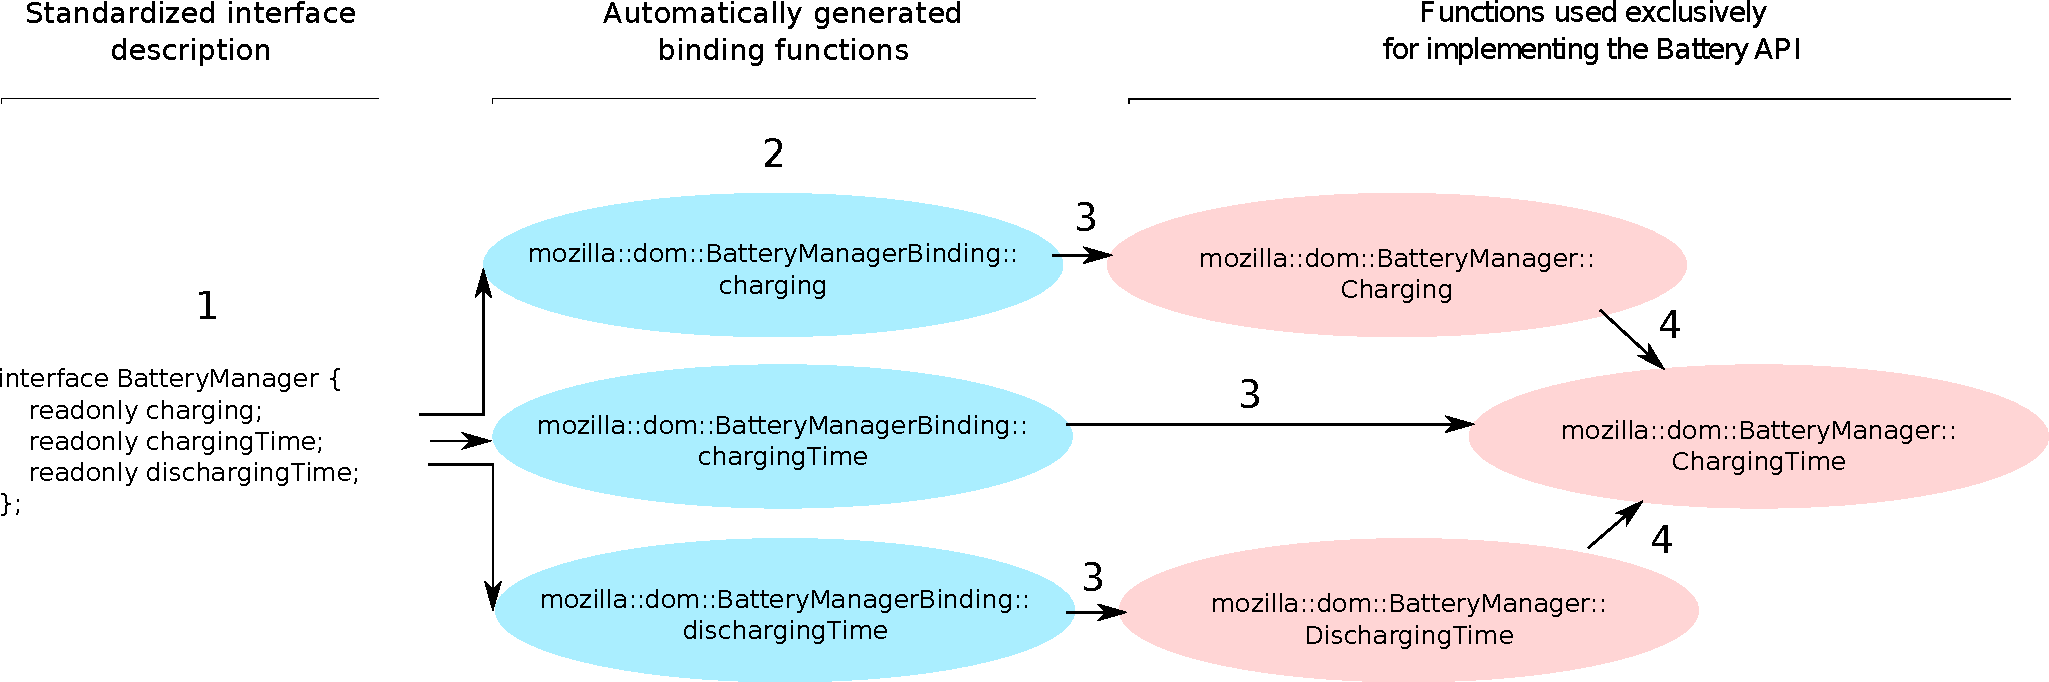
\includegraphics[width=\textwidth]{figures/prune_graph.pdf}
  \caption{An example of applying the graph pruning algorithm to a simplified version of the \textit{Battery API}.}
  \label{fig:prune-graph}
\end{figure}


Given the entry points in the call graph for each \WAPI feature, we used a
recursive graph algorithm to identify implementation code
associated with each standard. We
illustrate an example of this approach in
\ref{fig:prune-graph}.  In step 1, we programmatically extract the
standard's definitions for its binding functions, as we do here using a
simplified version of  the \textit{Battery API}. In step 2, we locate these
generated binding functions in the Firefox call graph (denoted by blue nodes).
By following the call graph, we identify implementation functions that are
called by the \textit{Battery API's} binding functions, denoted by pink nodes.
(step 3). If these pink nodes have no incoming edges other than binding functions, we
know they are solely in the code base because of the \WAS associated with
those binding functions.

The first iteration of the algorithm identifies two functions,
\texttt{Charging} and \texttt{DischargingTime}, as being
solely related to the \textit{Battery API} standard, since no
other code within the Firefox codebase contains a reference or call to those
functions.  The second iteration of the pruning process identifies the
\texttt{ChargingTime} function as also guaranteed to be solely related to the
\textit{Battery API} standard's implementation, since it is only called by
functions we know to be solely part of the \textit{Battery API}'s
implementation. Thus, the lines implementing all three of these pink
implementing functions are used to compute the \gls{eloc} metric for the
\textit{Battery API}.


\subsubsection{Third Party Libraries}
\label{cost-benefit:methodology:third-party-libraries}
This technique gives a highly accurate, lower bound measurement of lines of code
\emph{in the Firefox source} included only to implement a single \WAS.  It does not
include code from third-party libraries, which are compiled as a separate step
in the Firefox build process, and thus excluded from DXR's call-graph.

To better understand their use, we investigated how third party libraries are
used in the Firefox build process. In nearly
all cases, the referenced third party libraries are used in
multiples places in the Firefox codebase and cannot be uniquely
attributed to any single standard, and thus are not relevant to our per-standard \gls{eloc} counts.
%  These
% third-party libraries include code to handle multimedia (e.x. \textit{libav} and
% \textit{libpng}), advanced graphics operations (e.x. \textit{skia} and \textit{cairo}),
% or handling database operations (\textit{SQLite3}).  Such libraries are used
% across multiple standards, as well as in the non-Web API portions of Firefox,
% and thus are not relevant to our per-standard ELoC counts.

The sole exception is the \textit{WebRTC} standard, which uniquely uses over 500k
lines of third party code.  While this undercount is large, it is ultimately not significant
to our goal of identifying high-cost, low-benefit standards, as the high number
of vulnerabilities in the standard  (as found in CVEs) and comparatively high \gls{eloc} metric  already
flag the standard as being high-cost.

% All other
% standards either do not rely on a third partly library, or use a third party library
% that is shared with other parts of the Firefox base.

% amount of third-party code that is not used elsewhere in the codebase.  The
% \textit{WebRTC} standard uses the \textit{libjingle} and \textit{Chromium WebRTC}
% libraries, which make up 500k significant lines of code.  The result is that our
% ELoC metric dramatically undercounts the complexity \textit{WebRTC}
% adds to Firefox.
